\newpage
\section*{Supplementary materials}
\begin{figure*}[h]
\begin{center}
\centerline{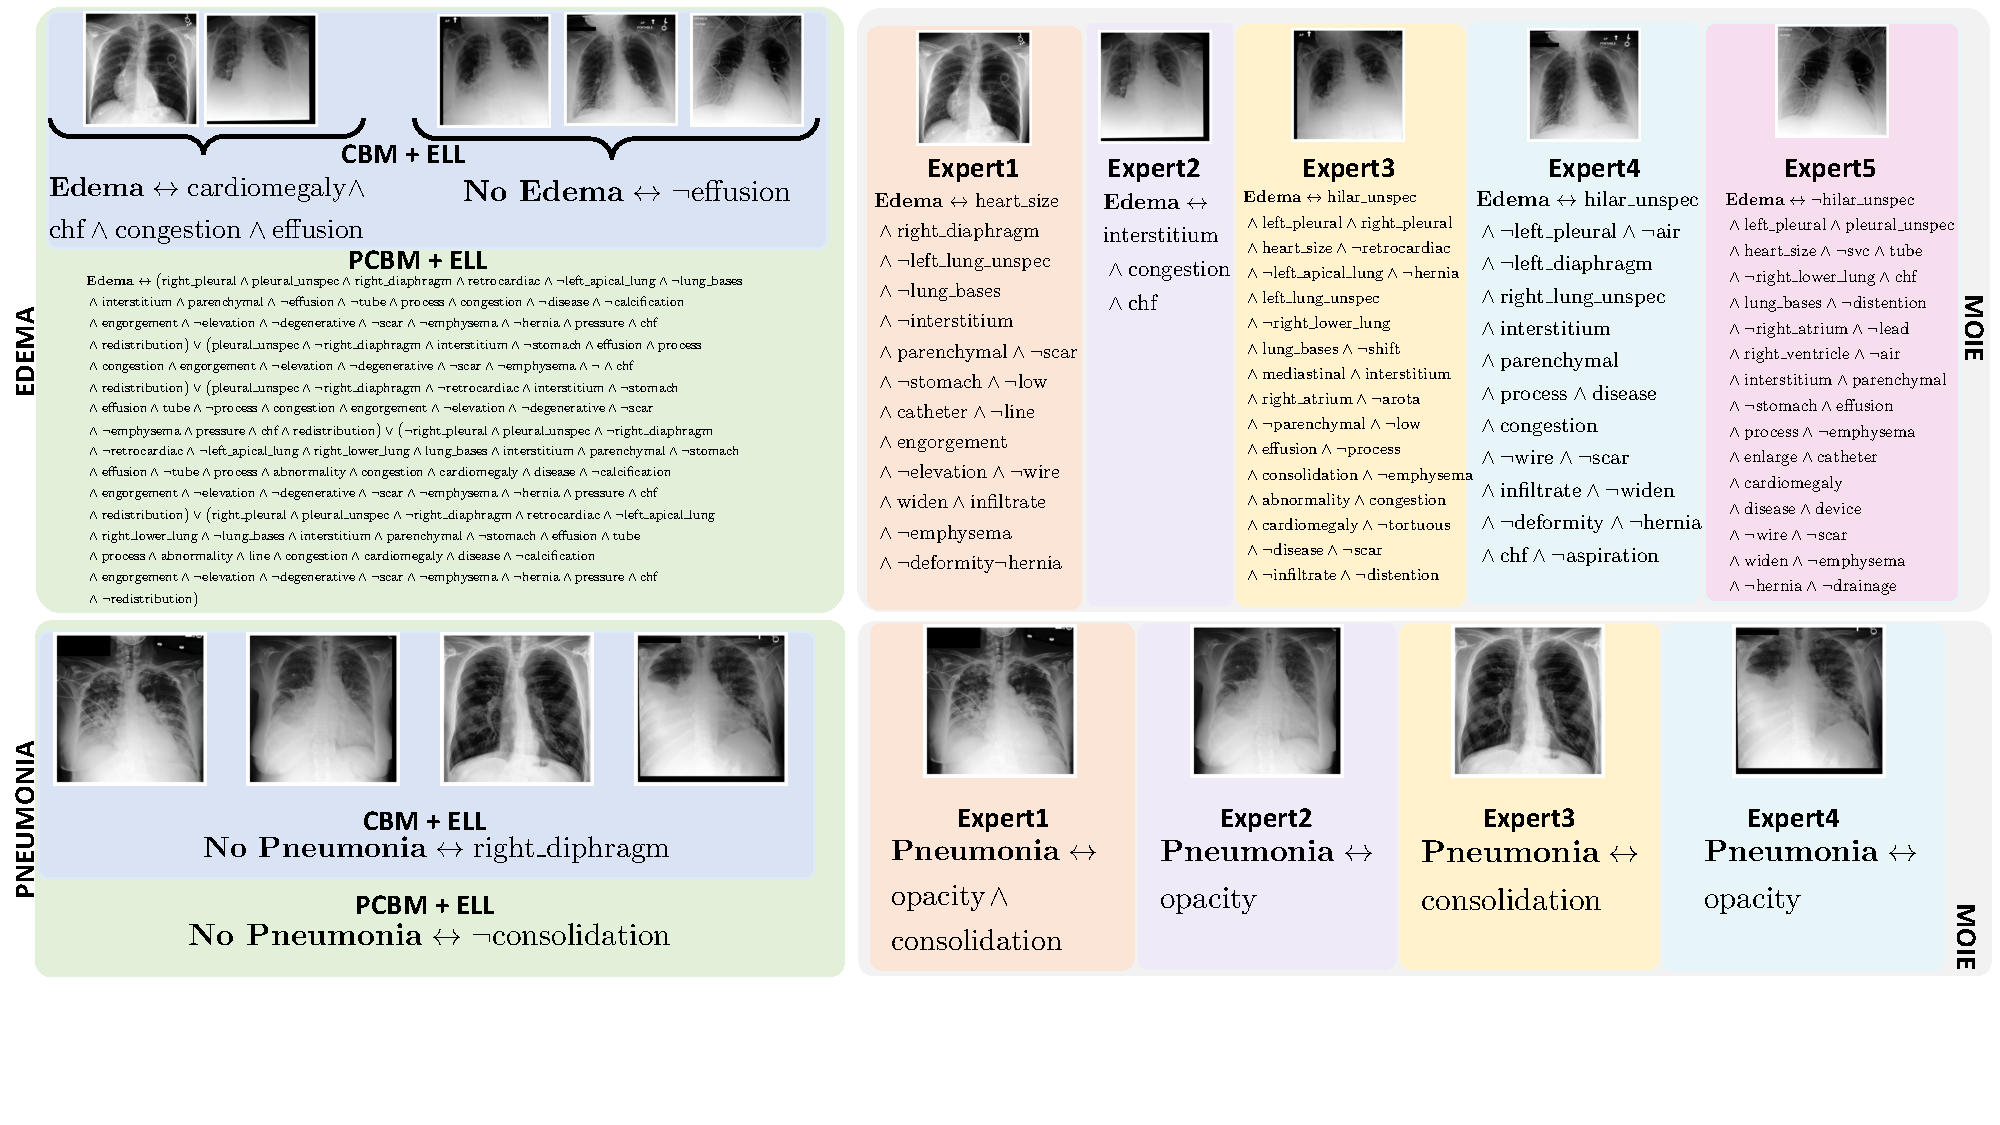
\includegraphics[width=\linewidth]{plots/supp/Supp_qual.pdf}}
\caption{Qualitative comparison of MoIE-CXR discovered concepts with the baseline for edema and pneumonia.}
\label{fig:expert_performance_cv_vit}
\end{center}
\end{figure*}

\begin{figure*}[h]
\begin{center}
\centerline{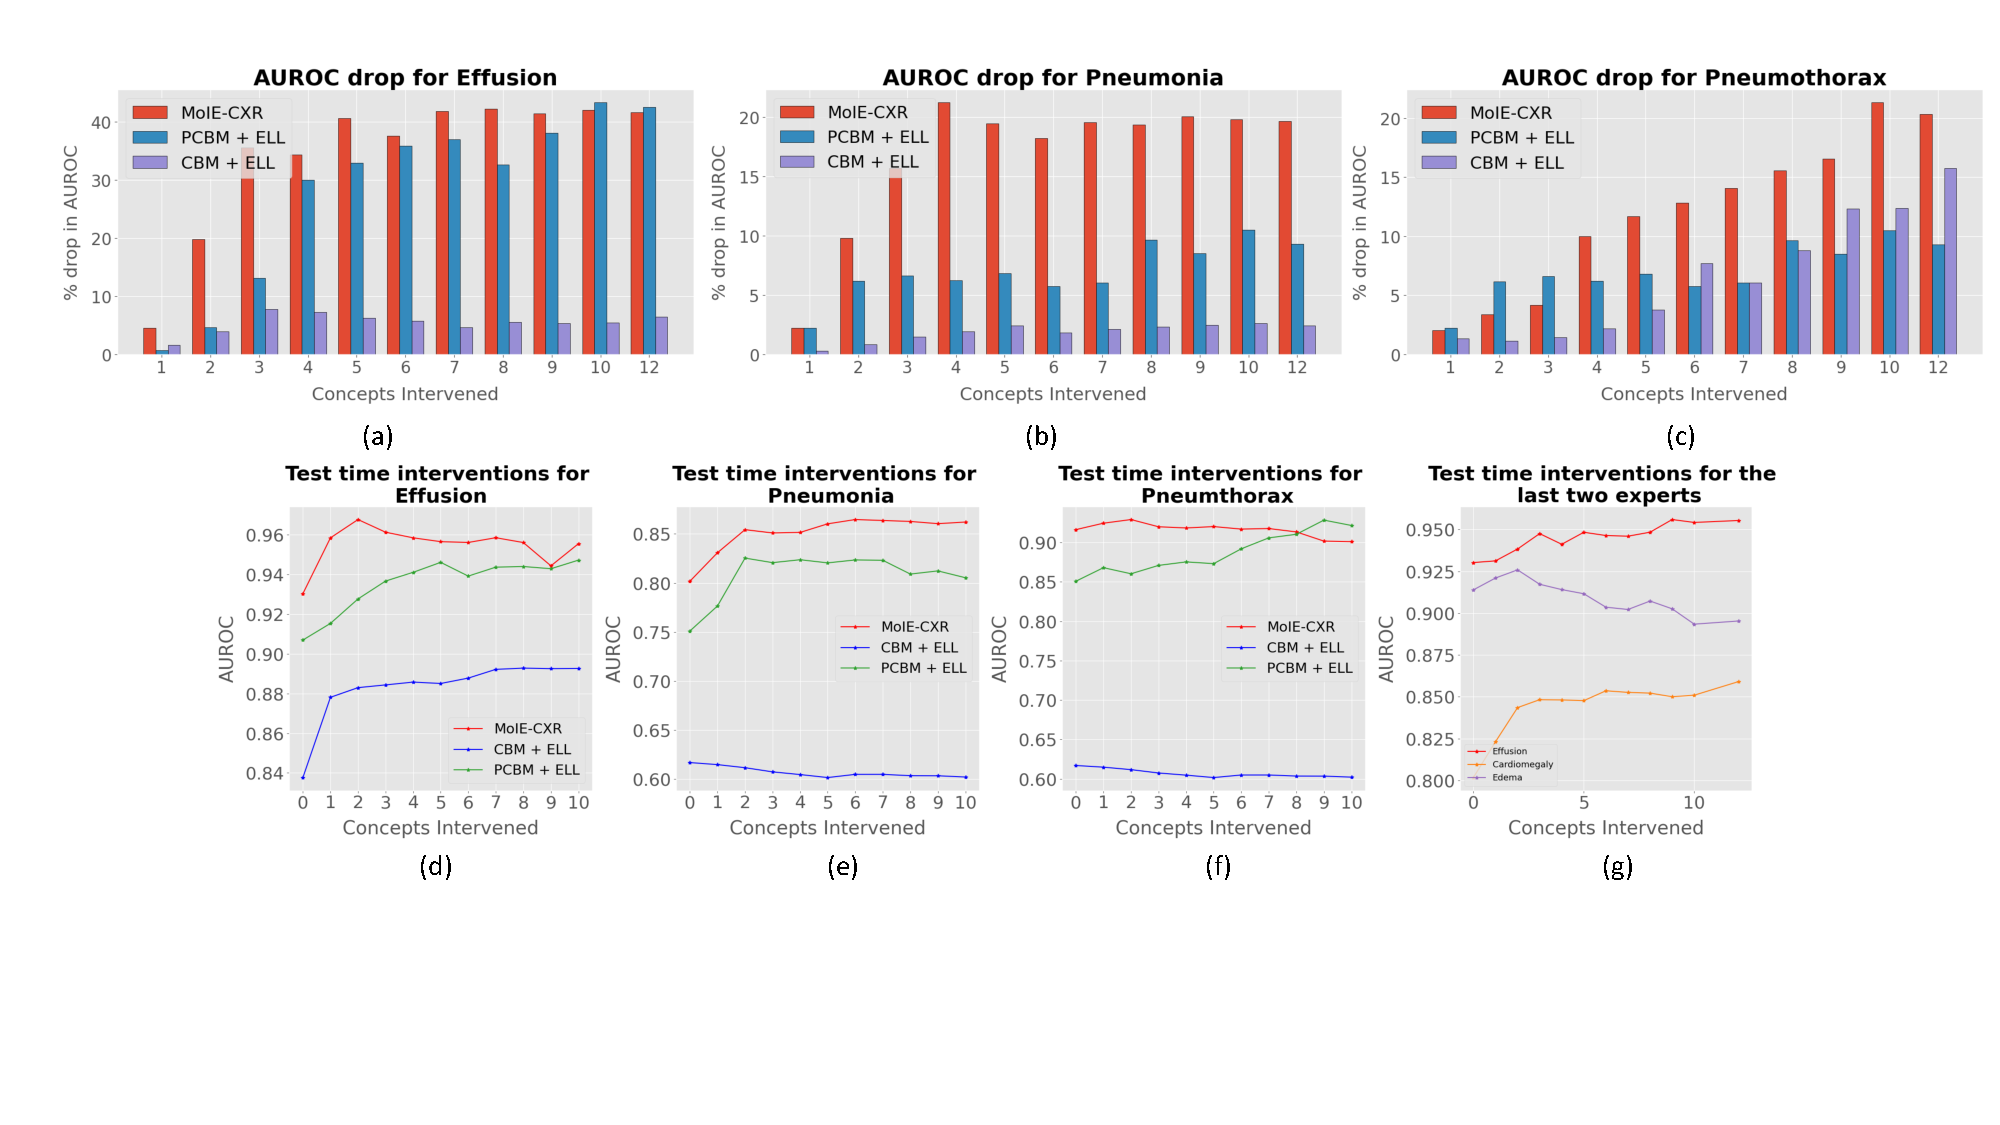
\includegraphics[width=\linewidth]{plots/supp/Supp_Quant_concepts.pdf}}
\caption{\textbf{(a-c):} Performance drop after zeroing out the concepts iteratively. The drop indicates the concepts to be more significant for prediction. \textbf{(d-g):} Test time interventions of concepts considering the ground truth concepts as an oracle on all samples (d-f), on the ``hard'' samples (g), covered by only the last two experts of MoIE-CXR.}
\label{fig:expert_performance_cv_vit}
\end{center}
\end{figure*}

\begin{figure*}[h]
\begin{center}
\centerline{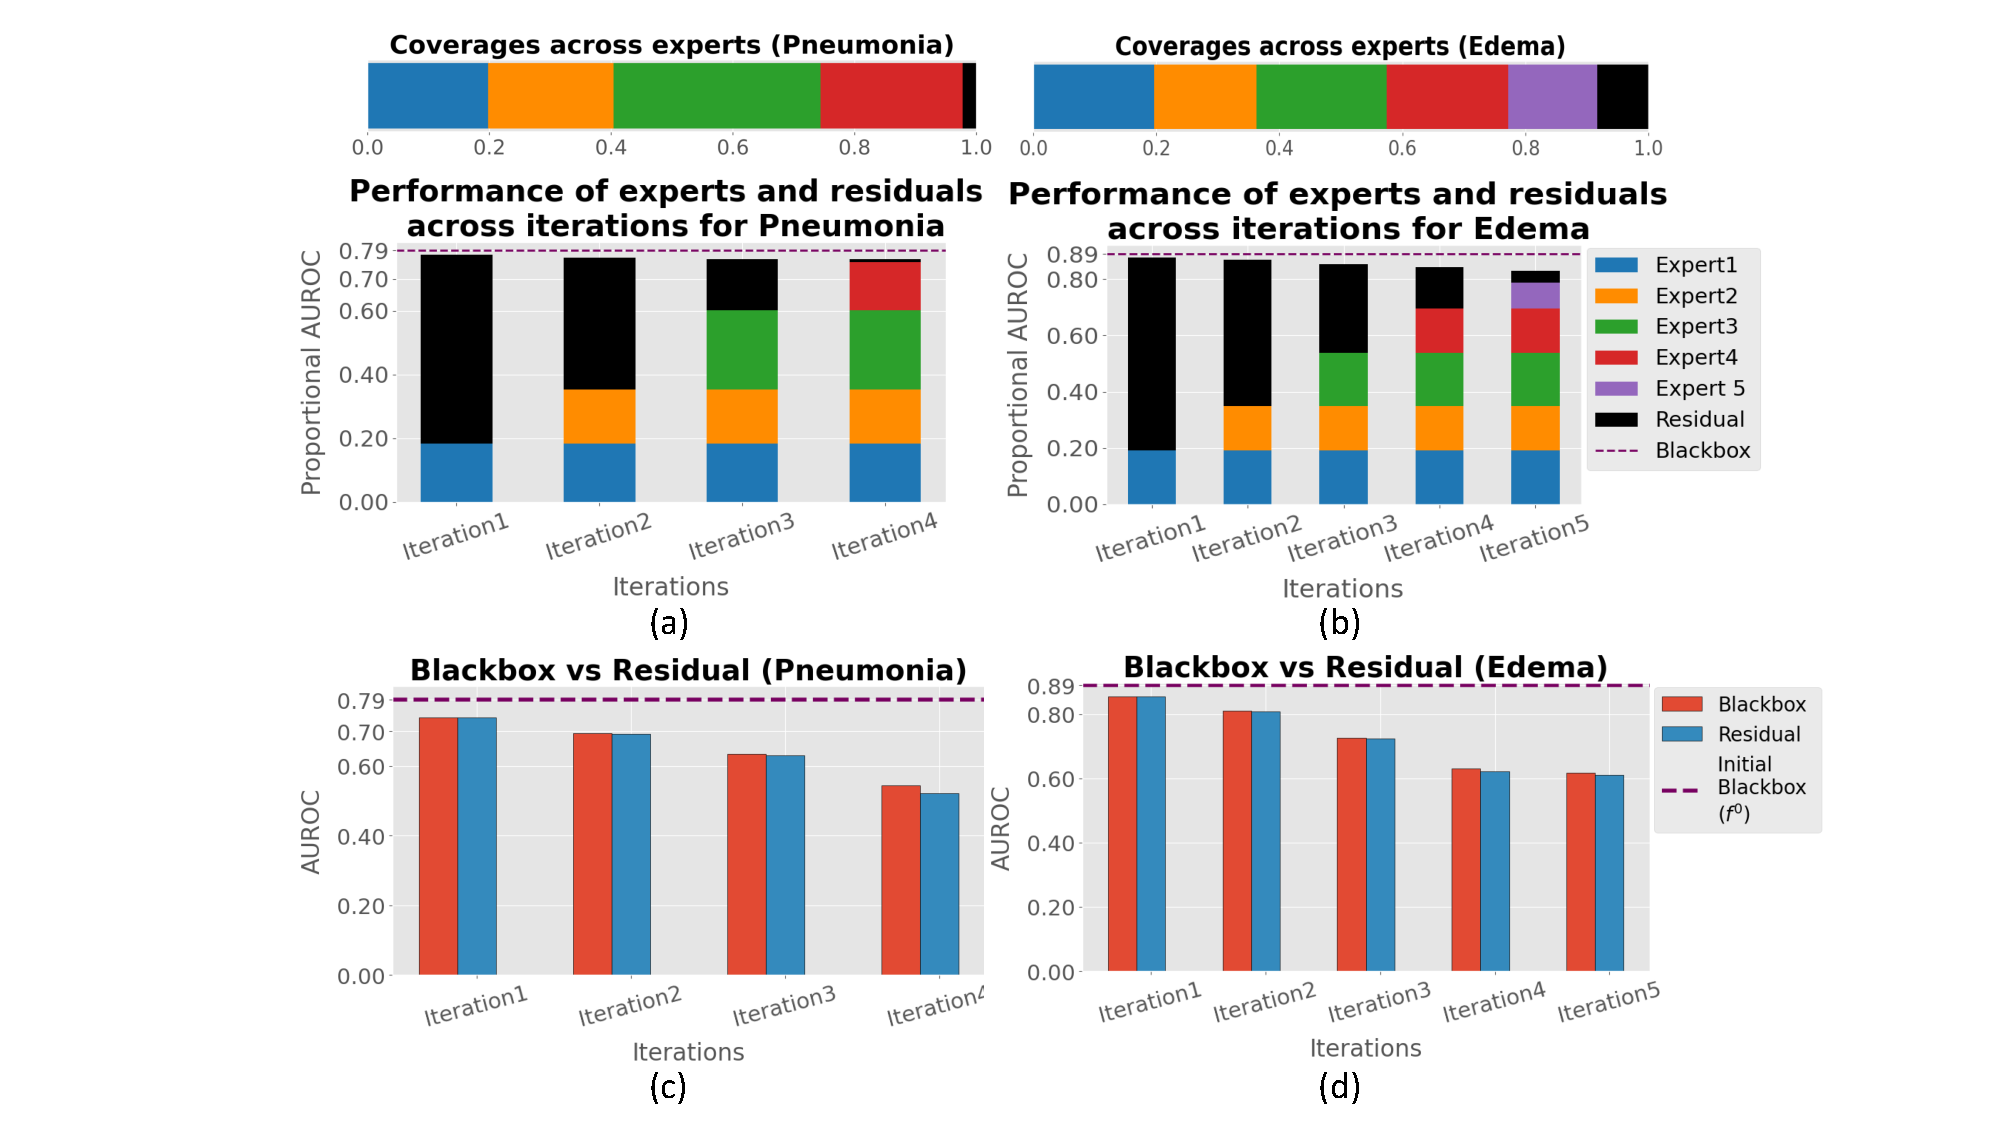
\includegraphics[width=\linewidth]{plots/supp/Supp_Experts.pdf}}
\caption{\textbf{(a-b)}: The performances of experts and residuals across iterations for pneumonia and edema. \textbf{(c-d)}: Performance comparison of the residuals and $f^0$ for the samples covered by the successive residuals.
}
\label{fig:expert_performance_cv_vit}
\end{center}
\end{figure*}

\begin{table}[H]
\caption{Hyperparameters of interpretable experts ($g$) for the dataset MIMIC-CXR.}
\label{tab:g_config_mimic_cxr}
\begin{center}
\begin{tabular}{l c c c c c }
\toprule 
    \thead{\textbf{Hyperparameter}} & 
    \thead{\textbf{Effusion}} & 
    \thead{\textbf{Cardiomegaly}} & 
    \thead{\textbf{Pneumothorax}} &
    \thead{\textbf{Pneumonia}} &
    \thead{\textbf{Edema}} \\
  
\midrule 
       Batch size & 1028 & 1028 & 1028 & 1028 & 1028   \\
       Learning rate & 0.01 & 0.01 & 0.01 & 0.01 & 0.01\\
       $\lambda_{lens}$ & 0.0001 & 0.0001 & 0.0001  & 0.0001 & 0.0001\\
       $\alpha_{KD}$ & 0.99 & 0.99 & 0.99 & 0.99 & 0.99 \\
       $T_{KD}$ & 20 & 20 & 20  & 20 & 20  \\
       hidden neurons & 30, 30 & 20, 20 & 20, 20 & 20, 20 & 20, 20 \\
       $\lambda_s$ & 96 & 1024 & 256 & 256 & 128   \\
       E-Lens ($T_{lens}$) & 7.6 & 7.6 & 10 & 10 & 7.6\\
       \# Expers ($T_{lens}$) & 5 & 4 & 5 & 4 & 5\\
\bottomrule
\end{tabular}
\end{center}
\end{table}

\end{document}
